\documentclass[12pt,fleqn]{standalone} 
\usepackage{bm}
 
\usepackage{graphicx}
\usepackage[dvipsnames]{xcolor}
\usepackage{tkz-linknodes}
\usepackage{tikz,pgfplots}
\pgfplotsset{compat=1.14}
\usetikzlibrary{arrows,shapes,intersections,angles,calc,quotes,through,decorations.text, positioning}



\begin{document}

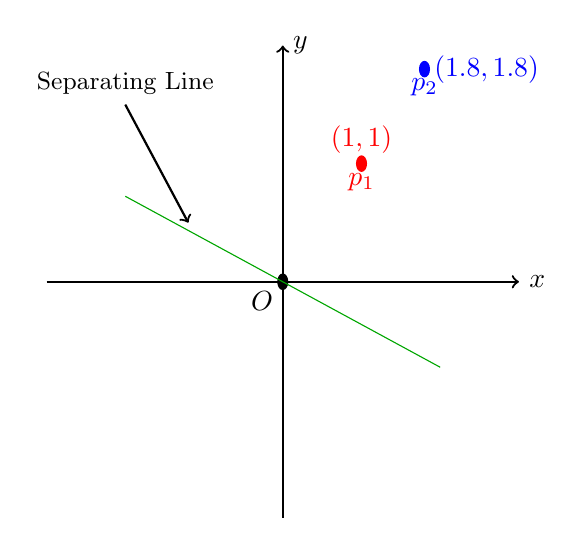
\begin{tikzpicture}[yscale=1.5]
\draw[thick,->] (-3,0) -- (3,0) node[right] {$x$};
\draw[thick,->] (0,-2) -- (0,2) node[right] {$y$};
\coordinate (O) at (0,0);
\coordinate (A) at (1,1);
\coordinate (B) at (1.8,1.8);
\fill(O) circle (2pt) node[below left] {$O$};
\fill[color=red] (A) circle (2pt) node[below,color=red] {$p_1$} node[above,color=red] {$(1,1)$};
\fill[color=blue] (B) circle (2pt) node[below, color=blue] {$p_2$}  node[right, color=blue] {$(1.8,1.8)$};

\draw [color=green!65!black,domain=-2:2] plot (\x, {(-0.362) * \x});
\draw[thick,->] (-2, 1.5) -- (-1.2,0.5) node[at start, above] {\small{Separating Line}};
\end{tikzpicture}

\begin{tikzpicture}[yscale=1.5]
\draw[thick,->] (-3,0) -- (3,0) node[right] {$x$};
\draw[thick,->] (0,-2) -- (0,2) node[right] {$y$};
\coordinate (O) at (0,0);
\coordinate (A) at (2,1);
\coordinate (B) at (-1,-1);
\fill(O) circle (2pt) node[below right] {$O$};
\fill[color=red] (A) circle (2pt) node[below,color=red] {$p_1$} node[above,color=red] {$(2,1)$};
\fill[color=blue] (B) circle (2pt) node[below, color=blue] {$p_2$}  node[above, color=blue] {$(-1,-1)$};
\draw [color=green!65!black,domain=-1:1] plot (\x, {(-1.179) * \x});
\draw[thick,->] (-2,0.5) -- (-0.5,0.6) node[at start, below] {\small{Separating Line}};
\end{tikzpicture}

\end{document}